%; whizzy chapter
% -initex iniptex -latex platex -format platex -bibtex jbibtex -fmt fmt
% 以上 whizzytex を使用する場合の設定。

%     Kansai Debian Meeting resources
%     Copyright (C) 2007 Takaya Yamashita
%     Thank you for Tokyo Debian Meeting resources

%     This program is free software; you can redistribute it and/or modify
%     it under the terms of the GNU General Public License as published by
%     the Free Software Foundation; either version 2 of the License, or
%     (at your option) any later version.

%     This program is distributed in the hope that it will be useful,
%     but WITHOUT ANY WARRANTY; without even the implied warranty of
%     MERCHANTABILITY or FITNESS FOR A PARTICULAR PURPOSE.  See the
%     GNU General Public License for more details.

%     You should have received a copy of the GNU General Public License
%     along with this program; if not, write to the Free Software
%     Foundation, Inc., 51 Franklin St, Fifth Floor, Boston, MA  02110-1301 USA

%  preview (shell-command (concat "evince " (replace-regexp-in-string "tex$" "pdf"(buffer-file-name)) "&"))
% 画像ファイルを処理するためにはebbを利用してboundingboxを作成。
%(shell-command "cd image200708; ebb *.png")

%%ここからヘッダ開始。

\documentclass[mingoth,a4paper]{jsarticle}
\usepackage{kansaimonthlyreport}
\usepackage[dvips]{xy}
\usepackage{ulem}

% 日付を定義する、毎月変わります。
\newcommand{\debmtgyear}{2014}
\newcommand{\debmtgdate}{23}
\newcommand{\debmtgmonth}{2}
\newcommand{\debmtgnumber}{82}

\def\fixme#1{{\color{red}{#1}}}

\begin{document}

\begin{titlepage}

% 毎月変更する部分、本文の末尾も修正することをわすれずに

 第\debmtgnumber{}回 関西 Debian 勉強会資料

\vspace{2cm}

\begin{center}
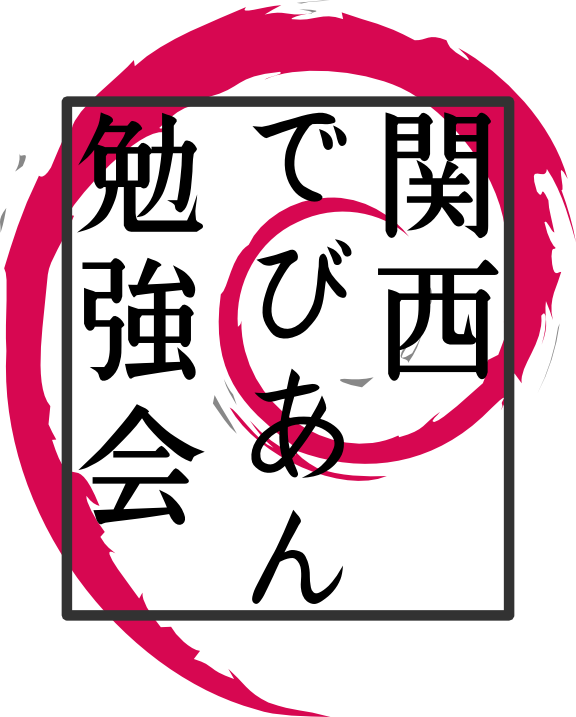
\includegraphics{image200802/kansaidebianlogo.png}
\end{center}

\begin{flushright}
\hfill{}関西 Debian 勉強会担当者 佐々木・倉敷・のがた・かわだ・八津尾 \\
\hfill{}\debmtgyear{}年\debmtgmonth{}月\debmtgdate{}日
\end{flushright}

\thispagestyle{empty}
\end{titlepage}

\dancersection{Introduction}{Debian JP}

\vspace{1em}

 関西Debian勉強会はDebian GNU/Linuxのさまざまなトピック
 (新しいパッケージ、Debian特有の機能の仕組、Debian界隈で起こった出来事、
 などなど)について話し合う会です。

 目的として次の三つを考えています。
 \begin{itemize}
  \item MLや掲示板ではなく、直接顔を合わせる事での情報交換の促進
  \item 定期的に集まれる場所
  \item 資料の作成
 \end{itemize}

 それでは、楽しい一時をお過ごしください。

\newpage

\begin{minipage}[b]{0.2\hsize}
 {\rotatebox{90}{\fontsize{80}{80}
{\gt 関西 Debian 勉強会}}}
\end{minipage}
\begin{minipage}[b]{0.8\hsize}
\hrule
\vspace{2mm}
\hrule
\setcounter{tocdepth}{1}
\tableofcontents
\vspace{2mm}
\hrule
\end{minipage}

\dancersection{最近のDebian関係のイベント報告}{Debian JP}

\subsection{第81回関西Debian勉強会}

81回目の関西Debian勉強会は2月23日(日)に、福島区民センターで行なわれまし
た。

もくもくがメインでしたが、LTおよび成果発表では、西山さんによる upstart と
docker の話、矢吹さんによるタイリングウィンドウマネージャ i3 の紹介、
佐々木さんによる systemd を入れた話、などが行なわれました。

\subsection{第110回東京エリアDebian勉強会}

110回目の東京エリアDebian勉強会は3月1日(土)にOSC 2014 Tokyo/Spring会場
にて出張開催されました。

岩松さんによる「Debian Update \& Debian のEFI/UEFI対応について」のセッ
ションとブース展示が行なわれました。

\subsection{第111回東京エリアDebian勉強会}

111回目の東京エリアDebian勉強会は3月15日(土)に株式会社スクウェア・エニッ
クス 会議室で行なわれました。

野島さんによる「debianとiphone5」のセッションともくもくの会の形式で行な
われました。

\subsection{Debian Project}

\subsubsection{Code of Conduct}
「[CTTE \#727708] Default init system for Debian\footnote{\url{https://lists.debian.org/debian-devel-announce/2014/02/msg00005.html}}」
あたりに端を発した一連の議論によってDebianでも「Code of Conduct(利用上
の注意)」が取り入れられようとしています。\footnote{\url{https://www.debian.org/vote/2014/vote_002}}

\subsubsection{Debian Installer Jessie Alpha1 release}

Debian インストーラーチームはDebian 8 ``Jessie'' のインストーラー アル
ファ1 をリリースしました。
\footnote{\url{https://www.debian.org/devel/debian-installer/News/2014/20140319}}

このインストーラーではデフォルトのデスクトップがXfceになっています。
これはtaskselの変更によるものですが、「とりあずXfceに変更しておくけど
2014年8月のDebConf14で再評価するぜ」となっているので、決定ではありません。

また、ia64とs390(s390xに置き換わった)はなくなりました。
あと、sparcもビルドできなかったので今のところありません。

\subsubsection{Bits from the Security Team}

セキュリティチームからの報告
\footnote{\url{https://lists.debian.org/debian-devel-announce/2014/03/msg00004.html}}
がありました。

この報告の中でSqueezeのLTSを提供できるのではないかと検討されています。
とはいえ「魔法のように空から降ってくるわけではない」ので協力者があらわ
れなければ実現しないでしょう。Squeezeのサポートは2014年5月で切れますの
でご注意を。

他にも、パッケージ名がリネームされた(ex. libfoo-ruby -$>$ ruby-foo)
のをどうやって追跡しようか(\debianbug{738172})、debsecanの開発に協力し
て欲しい、勧告に種別を含めなくなったよ、デフォルトコンパイラがGCC 4.9
になったら-fstack-protector-strongをdpkg-buildflagsに含めたい、などの
たくさんの話題がありますので目を通してみてください。

\subsubsection{パッケージ}

久しぶりにsidにご褒美がきたようです。

LVMを使っていてGRUBを2.02~beta2-7に更新すると起動しなくなるようです。
(\debianbug{735935})毎度のことながらGRUBの更新は鬼門ですね。
\newline

また、ca-certificates 20140223からCAcertの証明書が含まれなくなりました。
Mozillaのroot CAに要求する水準をCAcertが満たしていないことが原因のよう
です。(\debianbug{718434})
これによって\url{https://svn.debian.or.jp}などでサーバー証明書が検証
できなくなっていますが、どうしたものでしょうかね。

\subsubsection{その他}

「Bits from keyring-maint: Pushing keyring updates. Let us bury your old 1024D key!
\footnote{\url{https://lists.debian.org/debian-devel-announce/2014/03/msg00003.html}}
」ということで、1024bitの鍵は葬り去られていくようです。
\newline

Bublleさん\footnote{\url{http://www.perrier.eu.org/weblog/2014/02/25}}
によると、2/24に \debianbug{740000} が報告され3ヶ月ちょっとで10,000件増
えたそうです。(\debianbug{730000} は 2014/11/20)
この調子だと 800,000 件目は約18ヶ月後になりそうですが、
「800000th Bug Contest \footnote{\url{https://wiki.debian.org/800000thBugContest}}」
を見ると近いところを予想している人がいますがピタリと当たるでしょうか。
\newline

unstable/main に収録されているソースパッケージが 20,000 を超えました。
次の jessie は初のソースパッケージ 20,000 超えのリリースとなりそうです。
\footnote{\url{https://lists.debian.org/debian-devel/2014/03/msg00029.html}}

\dancersection{事前課題}{Debian JP}

今回の課題は以下の通りです。
\begin{screen}
  \begin{enumerate}
  \item %
    もくもくの会で行なう作業、質問などの課題を用意して教えてください。
    (電源とネットワーク(WiMAXなど)はありますが、それ以外の作業に必要な
    環境はご用意ください。)

  \item %
    前回(第81回)の勉強会に参加された方は、前回の作業や課題がその後どう
    なったか結果を教えてください。

  \item %
    LT 歓迎です。何かお話したい方はタイトルを下さい。
  \end{enumerate}
\end{screen}

参加者の皆さんの解答は以下の通りです:

\begin{prework}{ yyatsuo }
  \begin{enumerate}
  \item fcitx-skk の RFS します
  \item 前回不参加でした
  \item 特になし
  \end{enumerate}
\end{prework}

\begin{prework}{ 木下 }
  \begin{enumerate}
  \item
    \begin{enumerate}
    \item グリッドコンピューティング関連の調査・研究
      \begin{itemize}
      \item GlobusToolkitで何ができる?
        →AndroidOSのクロスコンパイルで使えたら嬉しいかも。
      \end{itemize}
    \item Eucalyptus(プライベートクラウドとして)の調査・研究
    \item Debian7 on PANDABOARDの調査・研究
      \begin{itemize}
      \item WiFiモジュール(On Board:TI製)の有効化
      \item GPUデバイスドライバの有効化
      \end{itemize}
    \end{enumerate}
  \item
    \begin{enumerate}
    \item Debian7 on PANDABOARDの調査・研究
      \begin{itemize}
      \item WiFiモジュール(USB)の接続

        実績:完了
      \item GPUデバイスドライバの有効化

        実績:保留
      \end{itemize}
    \end{enumerate}
  \end{enumerate}
\end{prework}

\begin{prework}{ 川江 }
  \begin{enumerate}
  \item 特にないです。ま、状況に応じてVMのdebianをインストールします。
  \item 前回はspiceの件ですが、課題のサーバのUEFIをupdateしたためにGRUB
    が飛んで、Debianを再インストールしている状況です。
  \item できれば4月ぐらいにkvmについてまとめたいと思っています。
  \end{enumerate}
\end{prework}

\begin{prework}{ 山城の国の住人 久保博 }
  \begin{enumerate}
  \item fpm2 の Segmentation fault が発生する不具合 \debianbug{647440}
    を修正するパッチを投稿できるように作業する。
  \item 前回は来ていませんでした。
  \end{enumerate}
\end{prework}

\begin{prework}{ Hideaki Oose }
  \begin{enumerate}
  \item ApacheSolrを使い情報検索の基礎を学ぶ。
  \item kfreebsd環境での無線LAN使用の可否を調べていますが、現在も未
    解決の状態です。同一環境下でネイティブFreeBSDと比較し可能性を検証
    中です。
  \end{enumerate}
\end{prework}

\begin{prework}{ murase\_{}syuka }
  \begin{enumerate}
  \item mruby-debianパッケージの更新
    \begin{itemize}
    \item 更新作法がよくわかってないので
    \end{itemize}
  \end{enumerate}
\end{prework}

\begin{prework}{ かわだてつたろう }
  \begin{enumerate}
  \item VCSで設定ファイルをどう管理しているのか聞いてみたい。
    あと、年度末事務作業を片付けたい。。
  \item すいません、寝込んでました。
  \end{enumerate}
\end{prework}

\begin{prework}{ 佐々木洋平 }
  \begin{enumerate}
  \item 毎度言ってる気がするが, tDiary と jekyll をなんとかしたい。
  \item 同上
  \item 多分、ネタは無いです。
  \end{enumerate}
\end{prework}

\begin{prework}{ lurdan }
  \begin{enumerate}
  \item python-social-auth のパッケージを作る予定です
  \item 3D Graphics のハードルが高すぎるので諦め気味です (MMP)
  \end{enumerate}
\end{prework}

\begin{prework}{ daism666 }
ワイヤレス環境構築にチャレンジしたいです。

Potato版を大学時代に触ってましたが、ここ八年触っておらず。

最近、WinXpを捨てこちらに戻ってきました。

よろしくお願いいたします。
\end{prework}

\begin{prework}{ 立川 勝宣 }
以前、一度参加させて頂きました。

3Dプリンター挑戦中です。
興味が有り、

参加させてください。

よろしくお願い致します。

実は、LTの意味解りません。
\end{prework}

\dancersection{Debian で楽しむ 3D プリンティング}{八津尾}

\dancersection{もくもくの会}{}

\dancersection{今後の予定}{Debian JP}

\subsection{関西Debian勉強会}

次回、第83回関西Debian勉強会は4月27日(日)に福島区民センターで開催します。

\subsection{東京エリアDebian勉強会}
第112回東京エリアDebian勉強会は4月19日(土)に場所は未定ですが開催予定です。

%
% 冊子にするために、4の倍数にする必要がある。
% そのための調整
%% \dancersection{メモ}{}
%% \mbox{}\newpage
%% \mbox{}\newpage
%% \mbox{}\newpage

\printindex
%\cleartooddpage

 \begin{minipage}[b]{0.2\hsize}
  \rotatebox{90}{\fontsize{80}{80} {\gt 関西 Debian 勉強会} }
 \end{minipage}
 \begin{minipage}[b]{0.8\hsize}

 \vspace*{15cm}
 \rule{\hsize}{1mm}
 \vspace{2mm}
 
\includegraphics[width=2cm]{image200502/openlogo-nd.eps}
 \noindent \Large \bfseries{Debian 勉強会資料}\\ \\
 \noindent \normalfont \debmtgyear{}年\debmtgmonth{}月\debmtgdate{}日 \hspace{5mm}  初版第1刷発行\\
 \noindent \normalfont 関西 Debian 勉強会 (編集・印刷・発行)\\
 \rule{\hsize}{1mm}
 \end{minipage}

\end{document}
